
%%% Local Variables: 
%%% mode: latex
%%% TeX-master: "report_dMRI_preprocessing.tex"
%%% End: 

\section{Coregistration: from native space to MNI space}
In the previous parts, tractographies were created using EuDX with FA from the raw data in dicom format. But, all these tractographies were initially in native space or space of scanner. Because every measurement has it own coordinator, it is very difficult for doctor or neuroscientist can compare, integrate or further studying them. They are needed to be warped into the common space. In the other way, registration is the process of transforming from native space into the coordinate system.

Image registration algorithms can also be classified according to the transformation models they use to relate the target image space to the reference image space. The first broad category of transformation models includes linear transformations, which include translation, rotation, scaling, and other affine transforms. Linear transformations are global in nature, thus, they cannot model local geometric differences between images. The second category of transformations is non-rigid or non-linear transformations. These transformations are capable of locally warping the target image to align with the reference image. Non-rigid transformations include radial basis functions (thin-plate or surface splines, multi-quadrics, and compactly supported transformations), physical continuum models (viscous fluids), and large deformation models (diffeomorphisms). 

The current known methodologies on this subject is that where Leemans et al.~\cite{leemans2006multiscale} uses the invariance of curvature and tortion under rigid registration along with procrustes analysis to co-register together different tractographies. Mayer et al. used iterative closest point applied to register preselected bundles (bundles of interest - BOI)~\cite{mayer2008bundles} ~\cite{mayer2007registration} and extended it using probabilistic boosting tree classifiers for bundle segmentation in~\cite{mayer2011supervised}. Durrleman et al.~\cite{durrleman2010registration} reformulate the tracks as currents and implemented a currents based registration, Zvitia et al.~\cite{zvitia2008adaptive},~\cite{zvitia2010coregistration}, used adaptive mean shift clustering to extract a number of representative fibermodes. Each fibre mode was assigned to a multivariate Gaussian distribution according to its population thereby leading to a Gaussian Mixture model (GMM) representation for the entire set of fibers. The registration between two fiber sets was treated as the alignment of two GMMs and is performed by maximizing their correlation ratio. Ziyan et al.~\cite{ziyan2007nonlinear} developed a nonlinear registration algorithm based on the log-Euclidean poly-affine framework~\cite{arsigny2009fast}, however this is not a direct tractography registration algorithm as they first create scalar volumes, therefore they don’t try to register the tracks as they are in their space. 

\begin{figure}
  \centering
  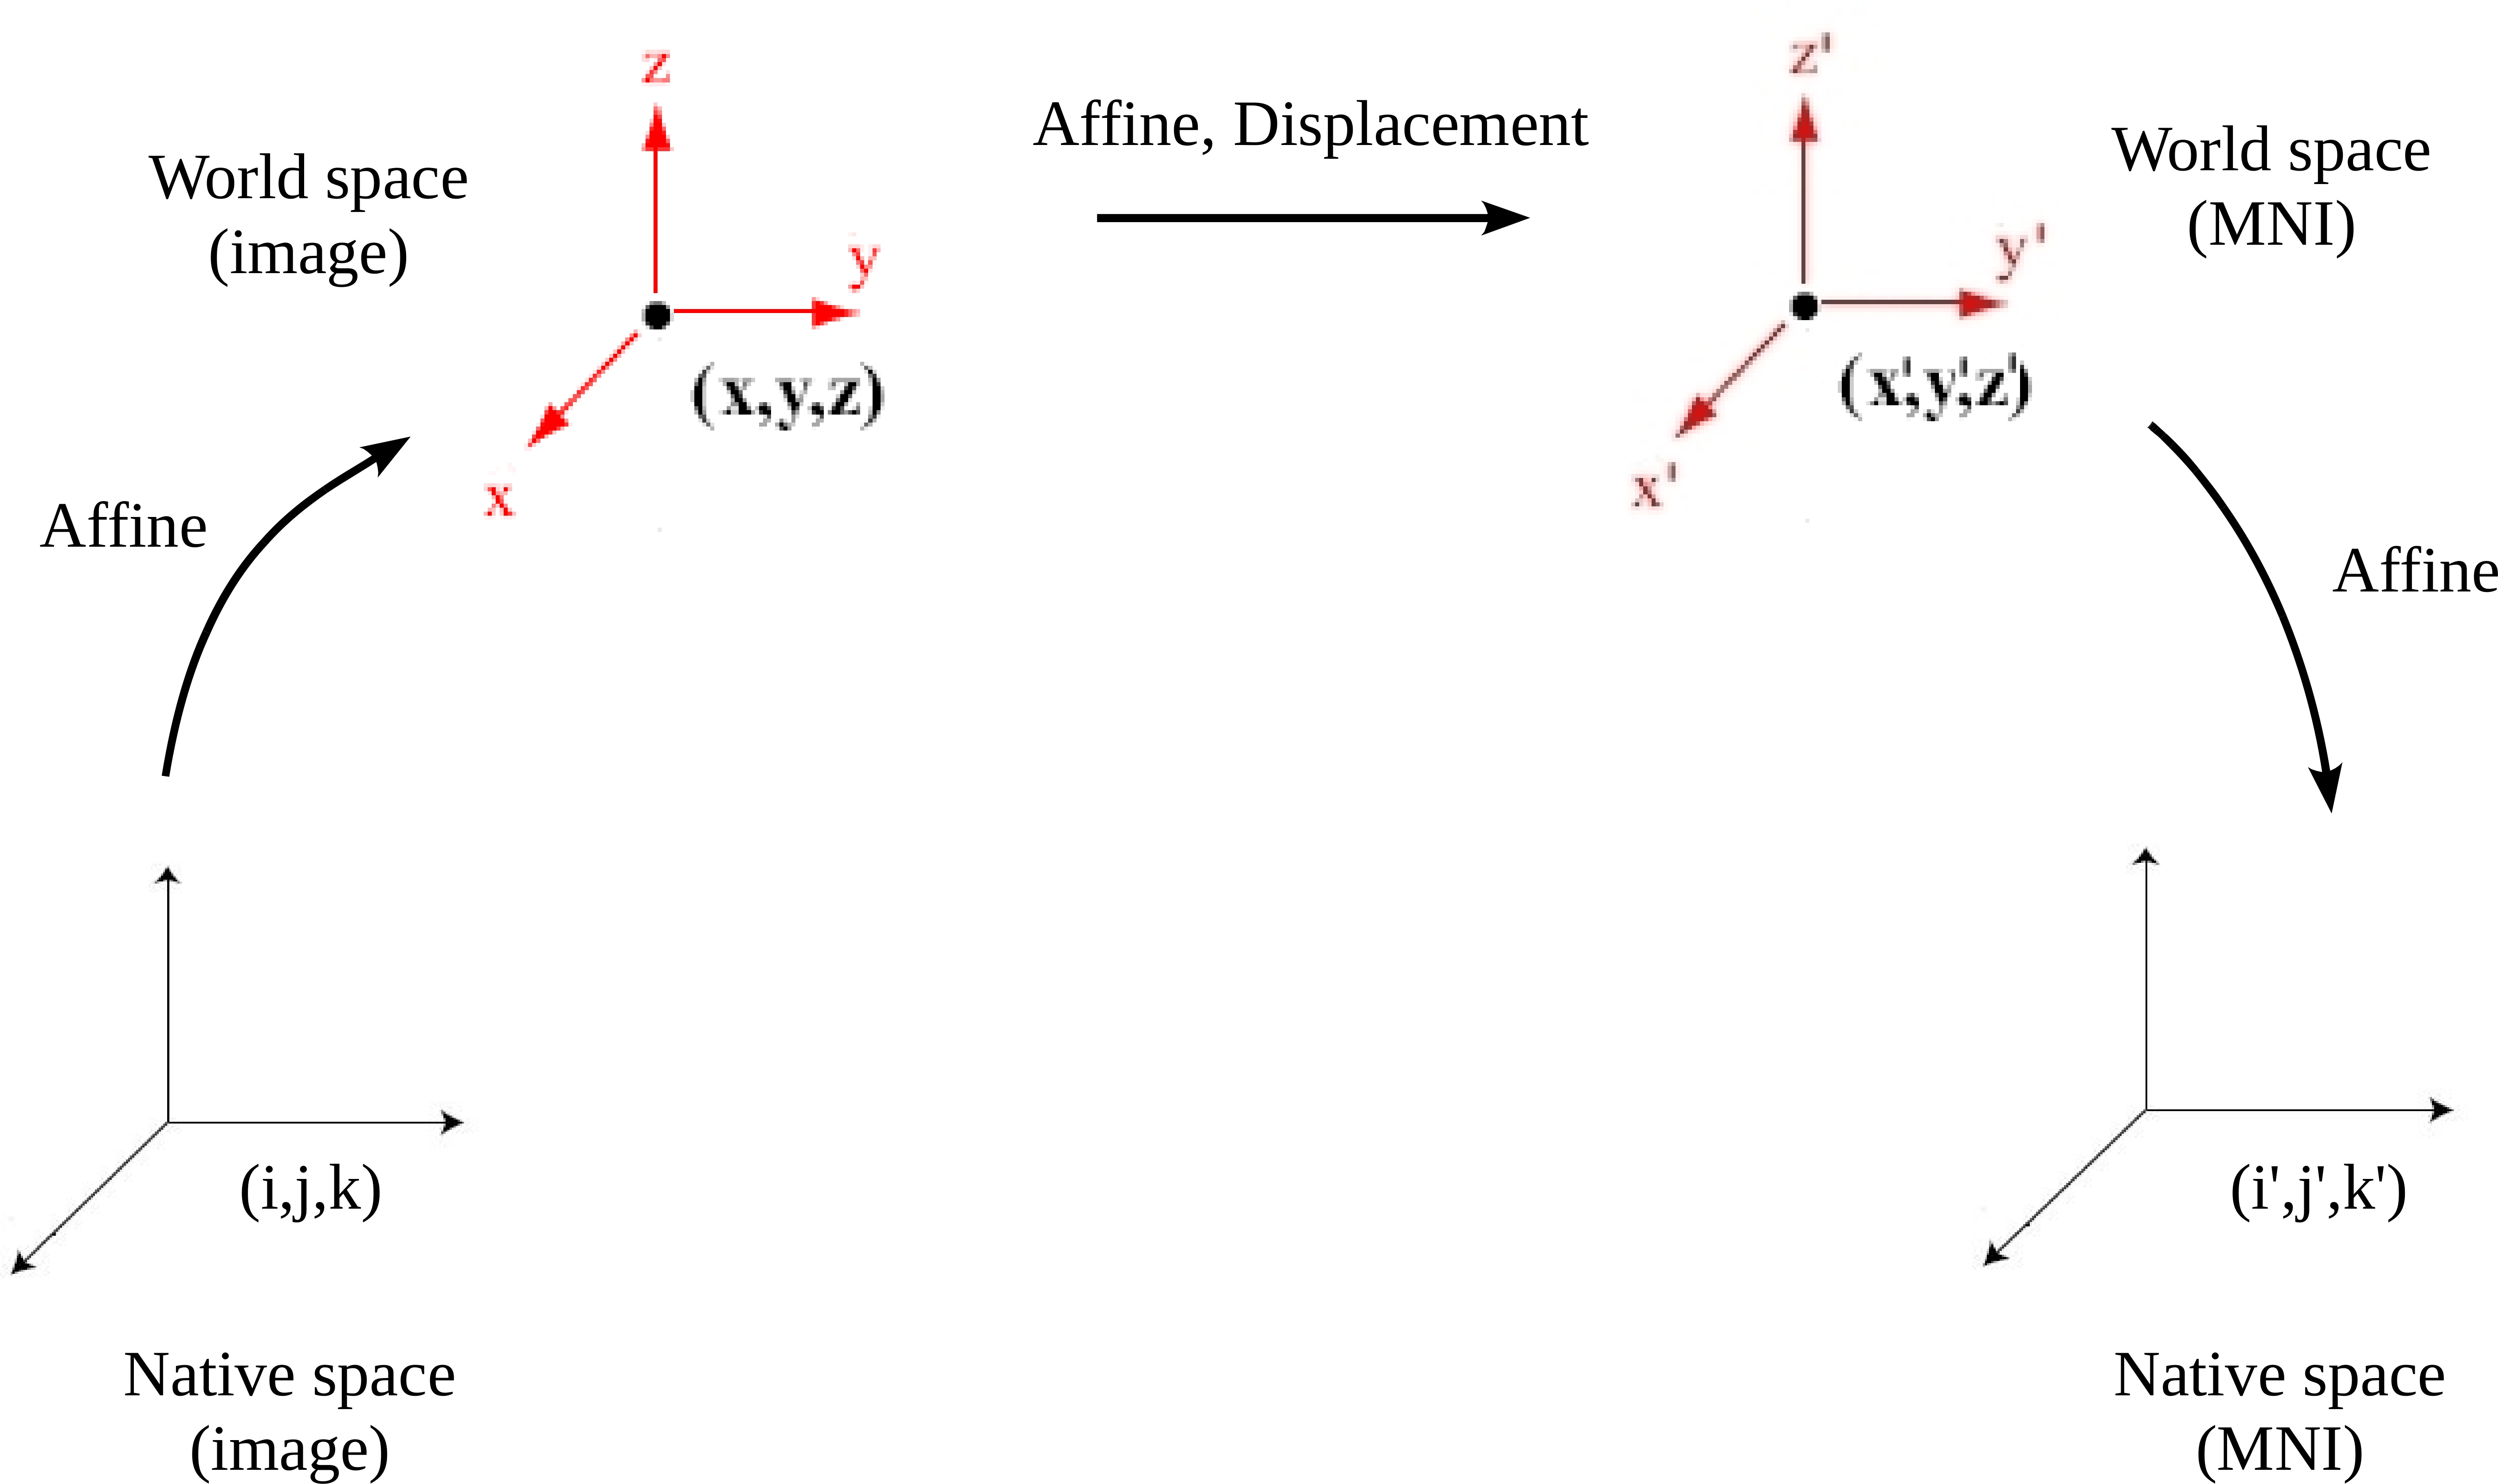
\includegraphics[width=13.7cm]{coregister.jpg}
  \caption{From native image space to MNI space.}
  \label{Fig:coregister}
\end{figure}

In this section, the goal is to warp the tractography from native space into MNI space (Montreal Neurological Institute)~\footnote{\url{http://www.mni.mcgill.ca/}}, a standard brain based on the averaging of 58 peoples, as in figure~\ref{Fig:coregister}. In contrast to the all the method mentioned before, in this implement we use FA registration mappings or affine transformation applied on tractography which is also most commonly used in the literature along with other tensor based methods~\cite{goh2006algebraic}. Native image (i,j,k) coordinates are mapped to native world coordinates by the affine of the image. In the same way the MNI image coordinates are mapped to MNI world coordinates through the MNI affine. The registration of the subject from native to MNI is about registering the native world to the MNI world. This can be done according to many models, e.g. affine transformation, rigid transformation or non-linear transformation, but always minimizing some loss function (e.g. correlation or mutual information)~\cite{zhu2002influence}. The data from the native image space are projected in native world and fitted to the template which is initially in MNI image space and through the affine in MNI world space.
\begin{center}===================================================\end{center}
\begin{lstlisting}[language=Prolog]
Coregistering
Input:  Tractography T in native space
Output: Tractography T in MNI space	
\end{lstlisting}
\begin{center}===================================================\end{center}
There are three steps that have been done for this processing. In order to co-registering the tractography, we must know two parameters: affine and displacement. Affine is a linear transformation matrix containing information about converting between image space and world space. And the displacement is a point wise mapping from native space to MNI space. It is technically very difficult with the FSL tools as they assume that these displacements will be applied only on volumetric data and not with point data as those used in tractographies. 
 
The question is how to compute these two parameters. From the section \textbf{\textit{reconstruction}}~\ref{sec:reconstruction}, we have the FA (fractional anisotrophy). This FA volume is also in native space. If there is an FA after warping in MNI space, it is possible to infer the affine and displacement. After that, these parameters can be used for registering the tractography. Due to this purpose, a standard template $FMRIB58_FA_1mm$ from the FSL toolbox was used as the reference volume. The FMRIB58 FA 1mm template has image coordinates (i,j,k) which corresponds to mm, because the size of one voxel is 1mm.

The transformation is usually done with FSL/FLIRT, which is linear, or FSL/FNIRT  which is non-linear. To get the affine transformation matrix, the linear transformation FLIRT is usually used:

\begin{python}
FLIRT
Input:  FA in native space
        Reference template 
        
Output: Affine matrix

flirt -ref FMRIB58_FA_1mm  -in <FA> -omat  <affine>
\end{python} 

or using non-linear transformation FNIRT

\begin{python}
FNIRT
Input:  FA in native space
        Linear Affine matrix
        Reference template 
        
Output: Nonlinear matrix

fnirt -in <FA> -aff <affine> -cout <nonlin>
\end{python} 

Actually, after some considerable effort we found a combination of flirt,fnirt,invwarp,fnirtfileutils and fnirtfileutils-withaff which gave us the correct displacements. As this being very technical we will not describe it further here but the code is available in module  (dipy.external.fsl)~\footnote{\url{http://nipy.sourceforge.net/dipy/index.html}}. The command line for this can be done as follow

\begin{python}
Create_displacements
Input:  FA in native space
        Linear Affine matrix
        Non-linear matrix
        Inverse warping matrix     
                
Output: Displacement
        Displacement with affine
create_displacements(<FA>,<Aff>,<Non>,<Inv>,<Disp>,<DispA>)
\end{python} 

After creating the displacement, the tractography will be applied to map them in the native space in the MNI space of voxel size 1 × 1 × 1mm3. Having all tractographies in MNI space is something very useful because we can now compare them against available templates or against each other and calculate different statistics. 

\begin{python}
Warp_displacements_tracts
Input:  Tractography in native space
	FA in native space
        Linear Affine matrix
        Inverse warping matrix
        Displacement
        Displacement with affine
        Reference template
                
Output: Warped tractography
warp_displacements_tracks(<T>,<FA>,<A>,<I>,<D>,<DA>,<R>,<TW>)
\end{python} 

\subsection{Linear vs. Non-linear registration: Issues}

We attempted non-linear registration of FA native into MNI/FA using FSL/FNIRT. The result is an affine matrix and a displacement
volume. This volume represents the displacements that each voxels has in order to match the template after the affine transformation. We
used affine and displacements on tractography data to warp it to MNI space. This is a meaningful operation since both the tractography and
the FA volume come from the same dMRI, i.e. they are in the same space. So far all good. The issues start when we need to nonlinearly
coregister T1 native into T1 MNI in order to superimpose T1 of the subject to his tractography in MNI space. The are 2 orders of issue:
\begin{enumerate}
\item Using FSL/FNIRT from T1 native to the MNI T1 template failed. The reasons are not clear but the result was visually not acceptable. This must be investigated more.
\item Even if nonlinear registration of T1 native to MNI T1 template succeed it is unclear whether the warping of T1 of the subject would be ``compatible'' to the warping of its tractography. T1 and tractography go along two different paths of registration and their results must be checked before accepting. It seems that until now no one attempted this nonlinear registration of both tractography and T1 that we attempted so there is no knowledge about this issue.
\end{enumerate}

Since nonlinear registration suffered this issue and we needed to have both T1 and tractography in the same space we reverted to linear
registration. So native FA/tractography was registered to MNI/FA template and then native T1 was registered to MNI T1. The result is
not great but still fine. Note that this whole registration problem is an open issue in neuroimaging. But in the case that you do not need to have T1 coregistered, e.g. when doing clustering, then nonlinear coregistration via FSL/FNIRT is good enough. Another option can be using the linear transformation provided by NiPy, and it will be evaluated later.

\subsection{Where is the Origin?}
The importance of this topic becomes evident when trying to show volumes and tractographies from MNI space within an OpenGL window.
In image $(i,j,k)$ space the origin is on one corner of the $3D$ matrix/volume, i.e. the $(0,0,0)$ cell/entry. When moving to world space each voxel, which is a cube, has its own origin in the centre of the cube. This last one is an assumption made by nibabel and it might be different in other tools (e.g. Trackvis assume that the origin of a voxel/cube is in one corner). In native world space the origin is defined by the MRI vendor but usually it is the center of the volume of the scan. In MNI world space the origin is in the middle of the brain. In MNI image space the origin, i.e. $(i,j,k)=(0,0,0)$ is again in one corner of the $3D$ matrix/volume.

 Given that the rotation and magnification parameters of the affine between MNI image and MNI world is $(-1.0, 1.0, 1.0)$, one voxel is $1mm$ and so the magnification is correct. But the origin is different: it is the corner of the volume for MNI image and center of the brain for MNI world, and a shift of half a volume is needed. More precisely the shift is $\frac{\mathrm{Vol}-1}{2}$. In figure ~\ref{Fig:sub1sub9coregister}, the red tractographies in top right corner at each sub-image are the original tractographies in native space. The green big ones are warped tractography. The sub-image on the left is 100 tract fibers of subject 1, while the right one shows the whole tractography of subject 9. Both subject 1 and subject 9 are collected from Cambrigde dataset.

\begin{figure}
  \centering
  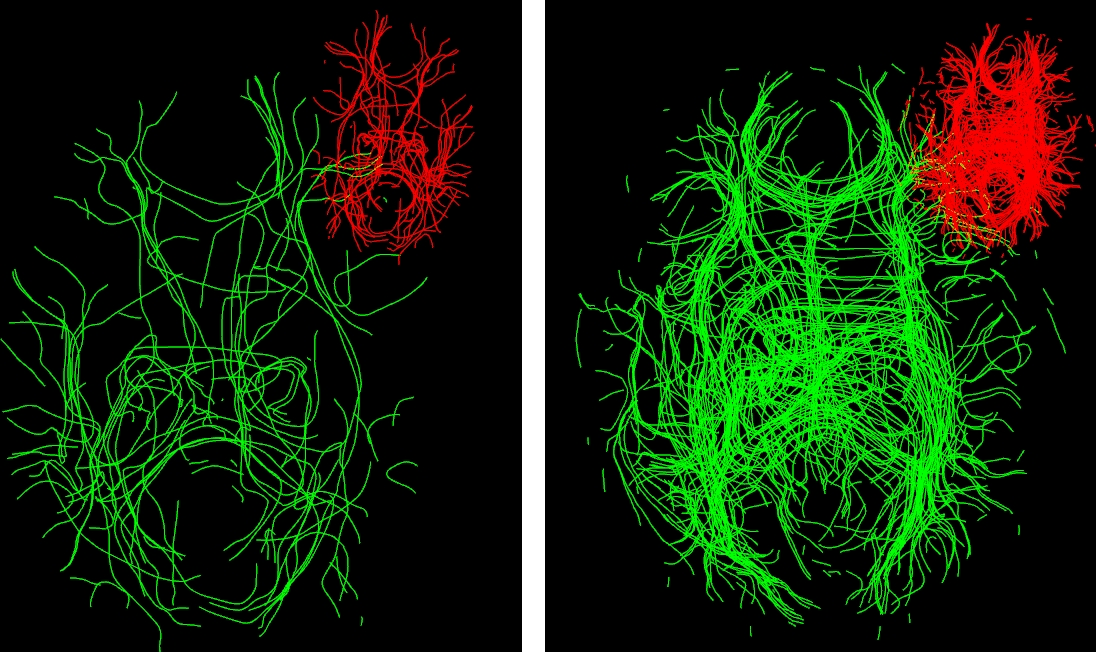
\includegraphics[width=10cm]{sub1_sub9_coregistering.jpg}
  \caption{Tractography before and after coregistration}
  \label{Fig:sub1sub9coregister}
\end{figure}



